\subsection{Single pulser}

\begin{figure}[htbp]
   \centering
   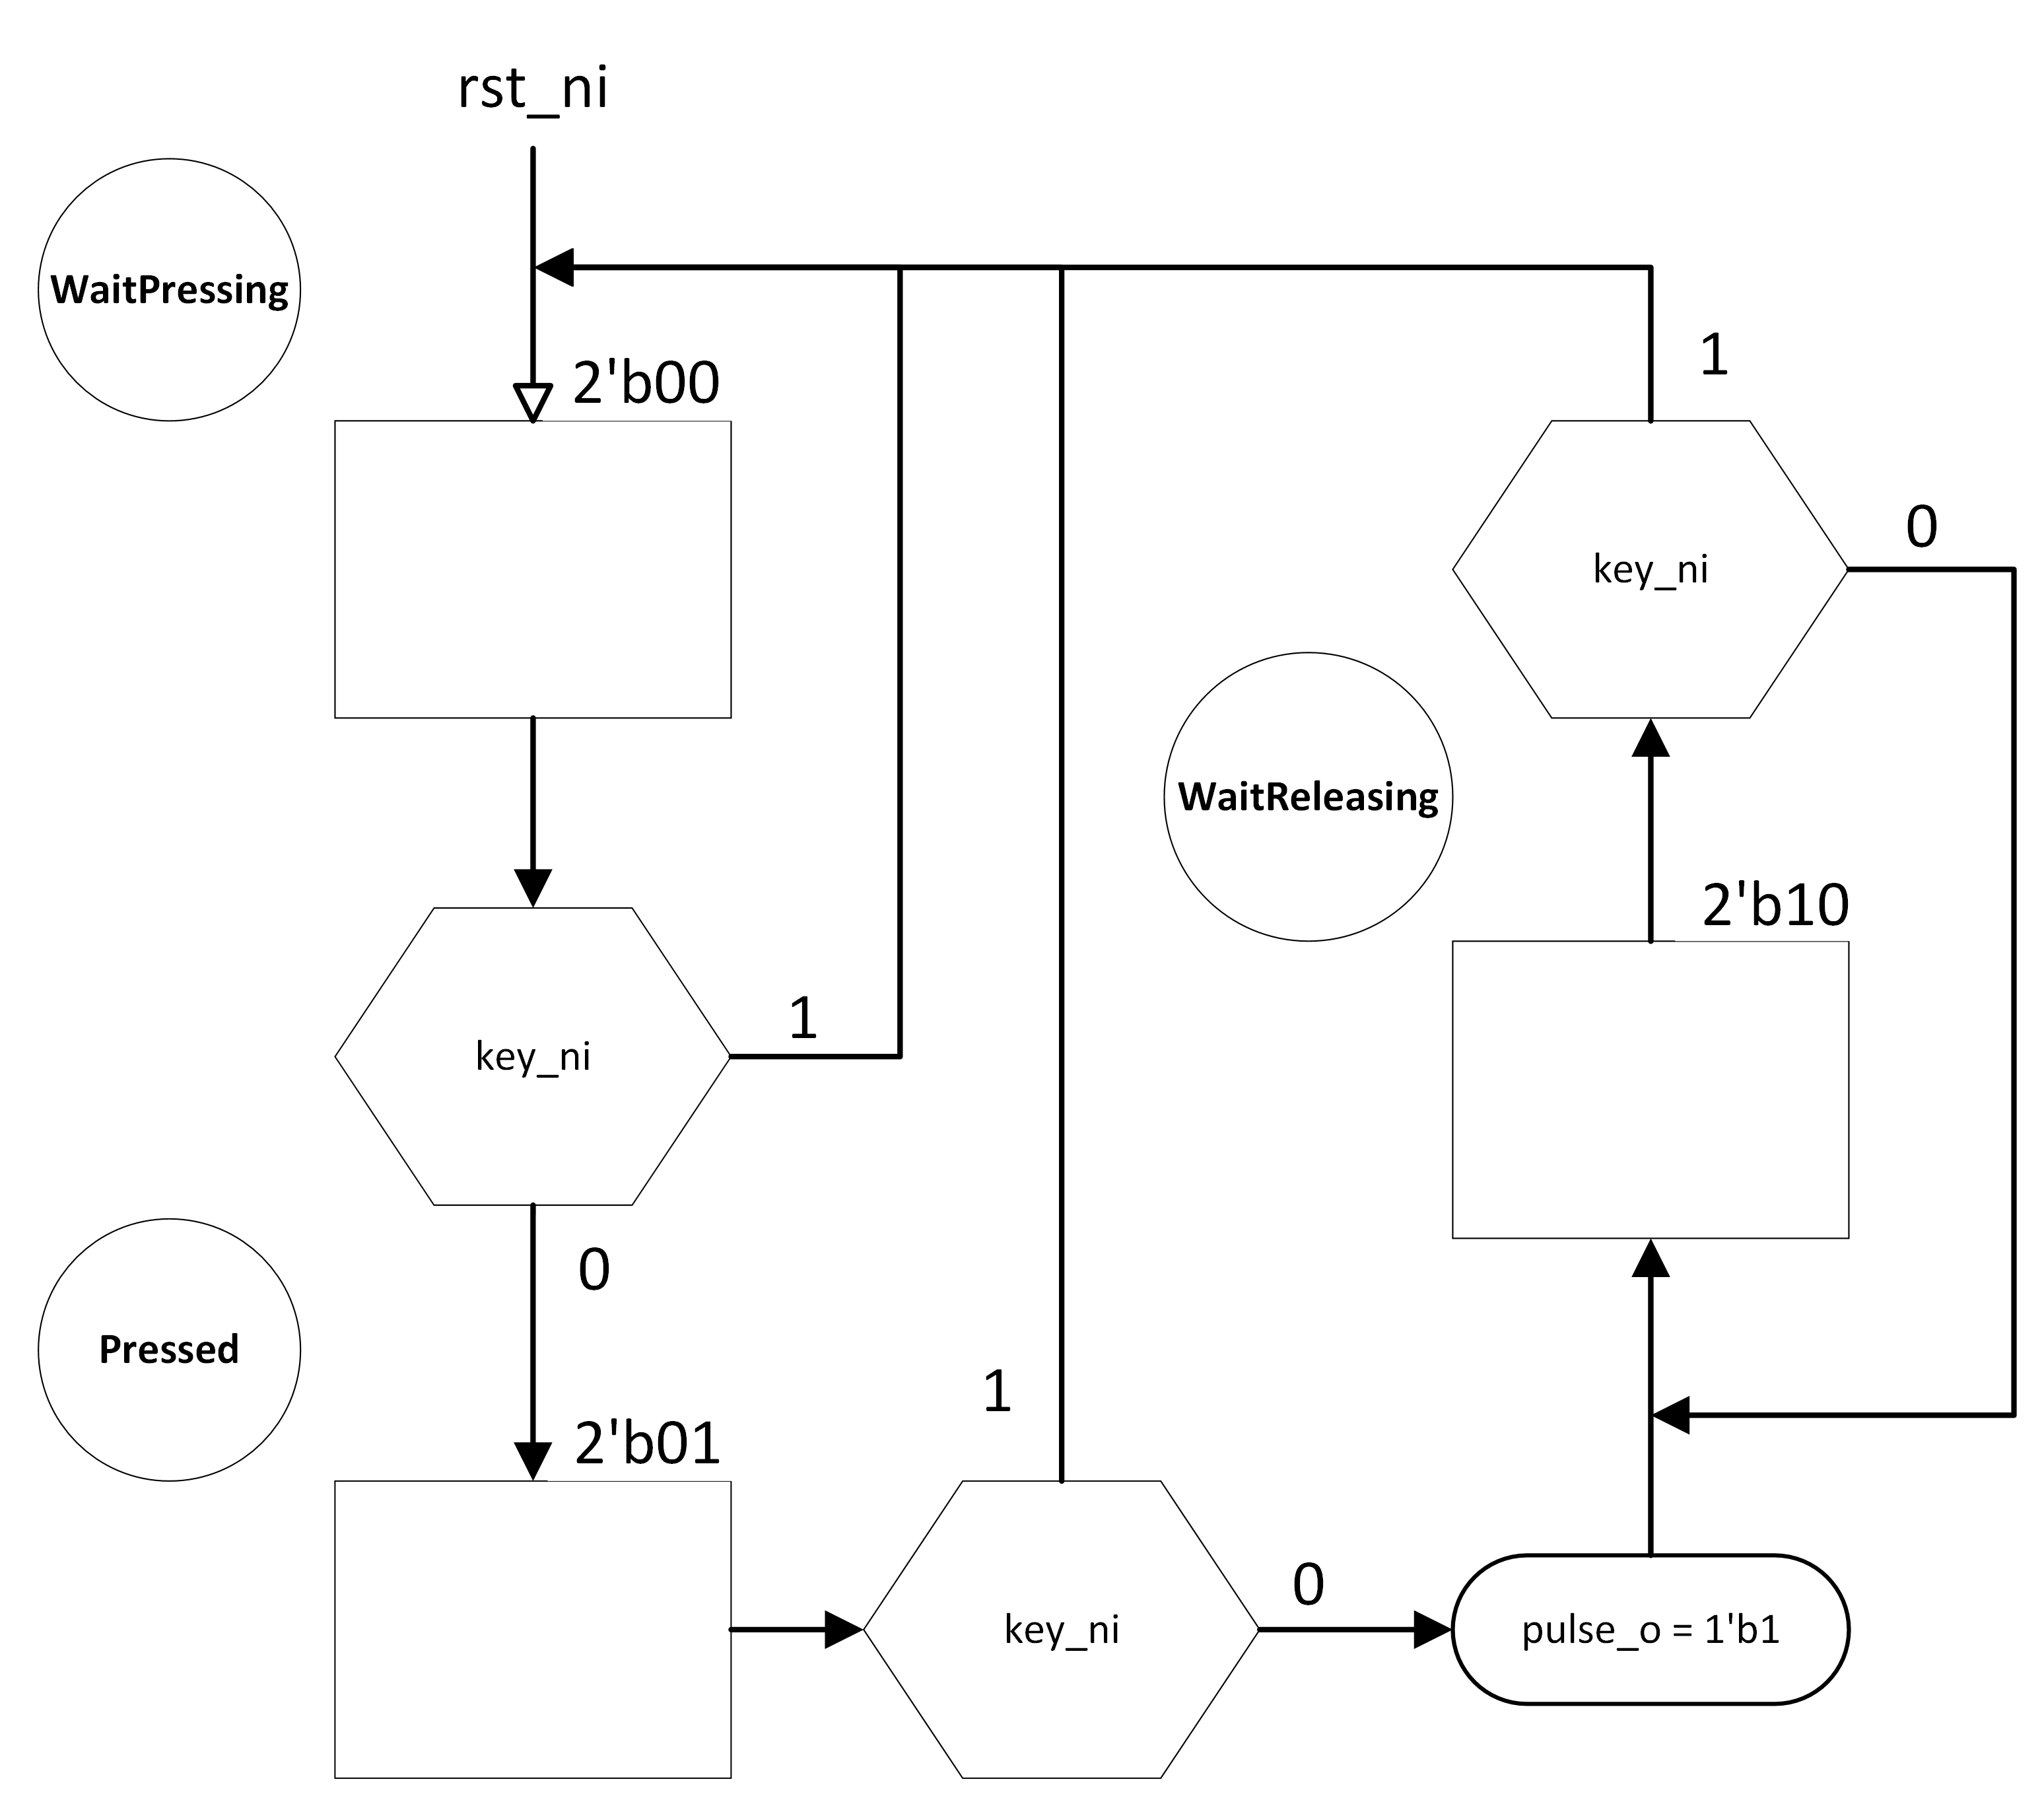
\includegraphics[width=\textwidth]{single_pulser_asm.png}
   \caption{ASM chart of the single pulser module.}
   \label{fig:single_pulser_asm}
\end{figure}

\begin{minted}[
   fontsize=\footnotesize,
   linenos,
   breaklines,
]{verilog}
module single_pulser (
   input clk_i,
   input rst_ni,
   input key_ni,
   output reg pulse_o
);

reg [1:0] state_d, state_q;
parameter WaitPressing = 2'b00;
parameter Pressed = 2'b01;
parameter WaitReleasing = 2'b10;

always @(posedge clk_i, negedge rst_ni)
   if (!rst_ni)
      state_q <= WaitPressing;
   else
      state_q <= state_d;

always @(state_q, key_ni) begin
   pulse_o = 1'b0;
   state_d = state_q;

   case (state_d)
      WaitPressing:
         if (!key_ni)
            state_d = Pressed;

      Pressed:
         if (!key_ni) begin
            pulse_o = 1'b1;
            state_d = WaitReleasing;
         end else
            state_d = WaitPressing;

      WaitReleasing:
         if (key_ni)
            state_d = WaitPressing;
   endcase
end

endmodule
\end{minted}

\begin{minted}[
   fontsize=\footnotesize,
   linenos,
   breaklines,
]{verilog}
module single_pulser_tb;

// Inputs
reg clk;
reg rst_n;
reg key_ni;

// Outputs
wire pulse_o;

single_pulser DUT (
   .clk_i(clk),
   .rst_ni(rst_n),
   .key_ni(key_ni),
   .pulse_o(pulse_o)
);

// Create a 50Mhz clock
always #10 clk = !clk;  // every ten nanoseconds invert

initial begin
   clk = 1'b0;
   rst_n = 1'b0;
   key_ni = 1'b1;
end

initial begin
   #20 rst_n = 1'b1;  // release reset

   // Long press
   #16;
   key_ni = 1'b0;
   #43;
   key_ni = 1'b1;

   // Brief contact
   #26;
   key_ni = 1'b0;
   #3;
   key_ni = 1'b1;
   #20;

   // Long press after brief contact
   #16;
   key_ni = 1'b0;
   #43;
   key_ni = 1'b1;

// Finish the Simulation
   #100;
   $finish;
end

endmodule
\end{minted}

\begin{figure}[htbp]
   \centering
   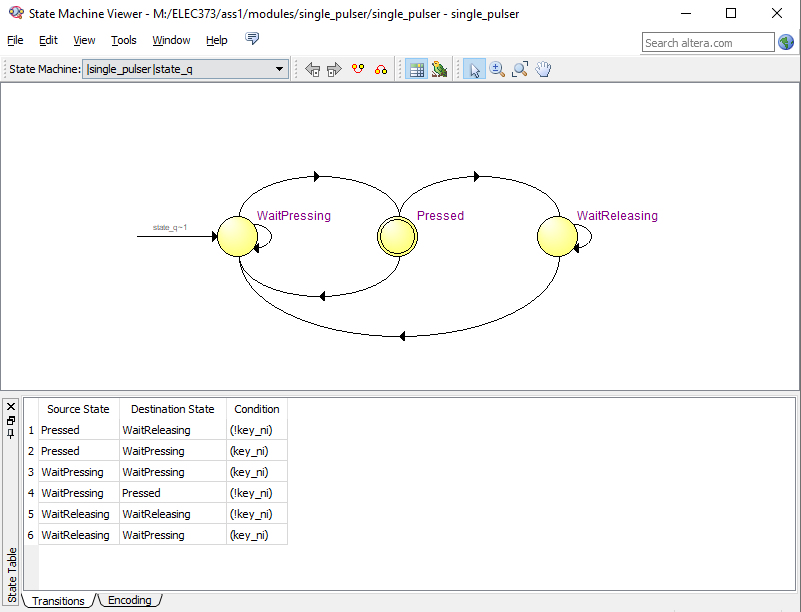
\includegraphics[width=\textwidth]{single_pulser_fsm.png}
   \caption{Quartus II state machine viewer shows the expected state machine of the single pulser after synthesis.}
   \label{fig:single_pulser_fsm}
\end{figure}

\begin{figure}[htbp]
   \centering
   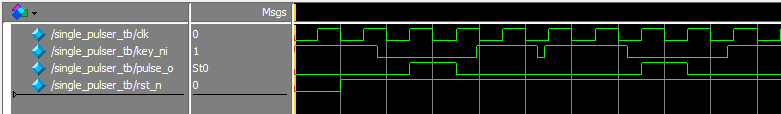
\includegraphics[width=\textwidth]{single_pulser_sim.png}
   \caption{Testbench simulation of the single pulser module.}
   \label{fig:single_pulser_sim}
\end{figure}

Fig.~\ref{fig:single_pulser_sim} illustrates the simulation test results of the single pulser module. Long lasting active-low signal was shortened into one pulse. Short signal was ignored. Short signal didn't affect the functionality of the signle pulser.
